% vim: ft=tex spell spelllang=en ts=2 sw=2
\cleardoublepage
\chapter{Analysis \& Design}

\todo[inline]{Consider moving this to previous chapter}

\section{Analyzing DWARF}

The \gls{DWARF} format was first developed by the Bell Labs for the
\verb|sdb| debugger of System V Unix. Nowadays the formal specification
is available under the GNU \gls{FDL}, and its new versions have been
discussed using public channels of communication, following a
community-oriented process. Downloadable copies of all the version of
the specification are available at {\small\url{http://dwarfstd.org}}.

In \gls{DWARF}, all the data provided by debugging information is stored in
a hierarchical tree-like structure, and each node of the tree is called
a \gls{DIE}. Each DIE consists of an identifying tag, and a series of
attributes. The tag specifies the class to which an entry belongs, and the
attributes define the characteristics of the entry. An entry, or a group of
entries together, provide a description of an entity in the corresponding
source code. The entries are contained in the \verb|.debug_info| and
\verb|.debug_types| sections of an object file.


%%%
%%% TikZ styles for DIE diagrams
%%%
\pgfdeclarelayer{background}
\pgfdeclarelayer{foreground}
\pgfsetlayers{background,main,foreground}

\tikzstyle{datablob} = [
  rectangle, rounded corners, drop shadow, draw=black, thick,
  text centered, minimum height=2em, minimum width=3em, fill=blue!20,
]
\tikzstyle{die}      = [start chain=going below, node distance=1mm]
\tikzstyle{dielabel} = [on chain]
\tikzstyle{dieitems} = [
  rectangle split, rectangle split parts=#1, rectangle split part align=left,
  thick, draw, fill=blue!10, on chain,
]
\tikzstyle{enumitems} = [
  rectangle split, rectangle split parts=#1, rectangle split part align=left,
  thick, rounded corners,
  color=black!50, fill=black!5, draw=black!50,
  minimum height=3em,
]
\tikzstyle{valuefrom} = [draw=black!50, thick, dashed]
\tikzstyle{arrow} = [draw, thick, >=triangle 45, ->]
\tikzstyle{datain} = [
  draw=black!80, thick, fill=blue!10, rectangle,
  text centered, minimum height=1.3em, text width=10em,
]
%%%
%%% End TikZ styles for DIE diagrams
%%%

\begin{figure}
  \centering
  \begin{tikzpicture}[die]
    \node[dielabel] (taglabel) {Tag};
    \node[dieitems=1] (tag) {\verb|DW_TAG_subprogram|};

    \node[dielabel] (attrlabel) {Attributes};
    \node[dieitems=3] (attributes) {
        \verb|DW_AT_type|
      \nodepart{two}
        \verb|DW_AT_sibling|
      \nodepart{three}
        \verb|DW_AT_…|
    };

    \node[datablob] (refdie2) [right=4cm of attributes] { };
    \node[datablob] (refdie1) [above=1mm of refdie2] { };
    \node  (refdieellipsis)   [below=1mm of refdie2] { ... };
    \node[datablob] (refdieN) [below=1mm of refdieellipsis] { };

    \node (refdieslabel) [above=3mm of refdie1] {DIEs referenced by offset};

    \path[arrow] (attributes.text east) -- (refdie1.west);
    \path[arrow] (attributes.two east) -- (refdie2.west);
    \path[arrow] (attributes.three east) -- (refdieN.west);

    \begin{pgfonlayer}{background}
      \node[datablob] (die) [fit=(taglabel) (attributes) (tag)] { };
      \node[fill=yellow!20, rectangle, rounded corners] (refdiesbg)
        [fit=(refdieslabel) (refdieN)] { };
    \end{pgfonlayer}

    \node (dielabel) [below=3mm of die] {DIE};
  \end{tikzpicture}

  \caption{DIE attribute references.}
  \label{fig:die-attr-references}
\end{figure}


The attributes can reference another DIE, as shown in
\autoref{fig:die-attr-references}, making it possible to create arbitrary
links between nodes of the tree. Those explicit links are used extensively to
group related entries together (for example the \verb|DW_TAG_formal_parameter|
entries, which describe the parameters of a function, are chained using
\verb|DW_AT_sibling| attributes), and to perform \gls{data-deduplication} of
the debug information (for example, instead of making a new entry for the
\mintinline{c}{int} type, only one is created and then referenced from other
entries).

\subsection{Debug Information Structure}
  \label{sec:debuginfo-structure}

This section provides simplified overview of the tree structure formed by the
debug information entries of a program, which is enough for the goals of this
project. For complete, detailed information, we refer to the DWARFv4
Specification~\cite{dwardspecv4}.


\subsubsection{Location of the Debug Information}

The contents of \gls{ELF} objects are described using \emph{segments}, and
\emph{sections}. Segments contain information used at runtime for the
execution of the code, and sections contain data about the code itself.
Sections contain data used \emph{offline} (i.e. not at runtime). Sections have
arbitrary names and contents. Debugging information is not strictly needed at
runtime for the execution of the program: it is considered ancillary, and is
stored in sections.

As per the specification, the DWARF debugging information must be stored in
the ELF objects in sections with the \verb|.debug_| prefix. Each one of those
sections stores a particular kind of information, as seen on
\autoref{tab:elf-dwarf-sections}. 


\begin{table}
  \centering\small
  \begin{tabular}{lp{0.65\textwidth}}
    \toprule
    Section & Contents \\
    \midrule
    \verb|.debug_types| & Stores DIEs for types. \\
    \verb|.debug_info| & Stores DIEs for executable program code (functions, mostly) \\
    \verb|.debug_line| & Maps of object code positions to source code line numbers \\
    \verb|.debug_pubnames| & Public function names and entry offsets in \verb|.debug_info| \\
    \verb|.debug_pubtypes| & Public type names and entry offsets in \verb|.debug_types| \\
    \verb|.debug_str| & String data (e.g. type, variable and function names) \\
    \bottomrule
  \end{tabular}
  \caption{Main ELF sections used to store DWARF debugging information}
  \label{tab:elf-dwarf-sections}
\end{table}


\subsubsection{Types}

A type is represented as a DIE with one of the following tags:

\begin{itemize}
  \item \verb|DW_TAG_base_type|
  \item \verb|DW_TAG_pointer_type|
  \item \verb|DW_TAG_typedef|
  \item \verb|DW_TAG_const_type|
  \item \verb|DW_TAG_array_type|
  \item \verb|DW_TAG_structure_type|
  \item \verb|DW_TAG_union_type|
  \item \verb|DW_TAG_enumeration_type|
\end{itemize}


\minisec{Base Types}

\begin{figure}
  \centering
  \begin{tikzpicture}[die]
    \node[dielabel] (taglabel) {Tag};
    \node[dieitems=1] (tag) { \verb|DW_TAG_base_type| };
    \node[dielabel] (attrlabel) {Attributes};
    \node[dieitems=2] (attributes) {
        \verb|DW_AT_byte_size|
      \nodepart{second}
        \verb|DW_AT_encoding|
    };

    \node[enumitems=1] (sizevalues) [right=4cm of tag] {\emph{size}};
    \node[enumitems=4] (encodingvalues) [below=1cm of sizevalues] {
        \verb|DW_ATE_signed|
      \nodepart{second}
        \verb|DW_ATE_unsigned|
      \nodepart{third}
        \verb|DW_ATE_float|
      \nodepart{fourth}
        \verb|DW_ATE_boolean|
    };

    \path[valuefrom] (attributes.text east) -- (sizevalues.west);
    \path[valuefrom] (attributes.second east) -- (encodingvalues.west);

    \begin{pgfonlayer}{background}
      \node[datablob] [fit=(taglabel) (attributes) (tag)] {};
    \end{pgfonlayer}
  \end{tikzpicture}
  \caption{DIE describing a base type.}
  \label{fig:die-base-type}
\end{figure}


Base types(\autoref{fig:die-base-type}) are represented by DIEs with
a \verb|DW_TAG_base_type| tag. This covers all the C/C++ numeric types: signed
and unsigned integers, floating point types (\mintinline{c}{float},
\mintinline{c}{double}), the \mintinline{c}{char} type, and the new
integer-based types of C99 (\mintinline{c}{_Bool}, \mintinline{c}{int32_t},
etc.)

The size of the values is given using a \verb|DW_AT_byte_size| attribute,
in bytes. Sizes are the same reported by the C \mintinline{c}{sizeof}
operator. A \verb|DW_AT_encoding| attribute specifies how the values are
used in the program. For example, \verb|DW_ATE_boolean|
corresponds with the \Mc|bool| type (or \Mc|_Bool|) in the
source program. The following table summarizes how C types are represented by
a base type DIE for the x86\_64 architecture (sizes may vary in other
architectures):

\begin{center}
  \begin{tabular}{lcl}
    \toprule
    C Type & \verb|DW_AT_byte_size| & \verb|DW_AT_encoding| \\
    \midrule
    \mintinline{c}{bool}               & 1 & \verb|DW_ATE_boolean| \\
    \mintinline{c}{char}               & 1 & \verb|DW_ATE_signed_char| \\
    \mintinline{c}{unsigned char}      & 1 & \verb|DW_ATE_unsigned_char| \\
    \mintinline{c}{short int}          & 2 & \verb|DW_ATE_signed| \\
    \mintinline{c}{unsigned short int} & 2 & \verb|DW_ATE_unsigned1| \\
    \mintinline{c}{int}                & 4 & \verb|DW_ATE_signed| \\
    \mintinline{c}{unsigned int}       & 4 & \verb|DW_ATE_unsigned| \\
    \mintinline{c}{long int}           & 8 & \verb|DW_ATE_signed| \\
    \mintinline{c}{unsigned long int}  & 8 & \verb|DW_ATE_unsigned| \\
    \mintinline{c}{float}              & 4 & \verb|DW_ATE_float| \\
    \mintinline{c}{double}             & 8 & \verb|DW_ATE_float| \\
    \mintinline{c}{long double}        & 16& \verb|DW_ATE_float| \\
    \bottomrule
  \end{tabular}
\end{center}

The rest of C/C++ base types are defined as aliases of these
using \mintinline{c}{typedef}.


\minisec{Pointer Types}

\begin{figure}
  \centering
  \begin{tikzpicture}[die]
    \node[dielabel] (taglabel) {Tag};
    \node[dieitems=1] (tag) {\verb|DW_TAG_pointer|};
    \node[dielabel] (attrlabel) {Attributes};
    \node[dieitems=1] (attributes) {\verb|DW_AT_type|};

    \node[dielabel] (rtaglabel) [right=3cm of tag, yshift=-3.5mm] {Tag};
    \node[dieitems=1] (rtag) {\verb|DW_TAG_pointer|};
    \node[dielabel] (rattrlabel) {Attributes};
    \node[dieitems=1] (rattributes) {\verb|DW_AT_type|};

    \node[datablob] (basedie) [right=2cm of rattributes] {Type DIE};

    \path[arrow] (rattributes.text east) -- (basedie);

    \begin{pgfonlayer}{background}
      \node[datablob] (die) [fit=(taglabel) (attributes) (tag)] {};
      \node[datablob] (rdie) [fit=(rtaglabel) (rattributes) (rtag)] {};
    \end{pgfonlayer}

    \path[arrow] (attributes.text east) -- (rdie.west);
  \end{tikzpicture}
  \caption{DIEs describing a Pointer-to-pointer-to type.}
  \label{fig:die-pointer-type}
\end{figure}

Pointer types (\autoref{fig:die-pointer-type}) are represented by DIEs with
a \verb|DW_TAG_pointer_type| tag, and a lone \verb|DW_AT_type| attribute
points to the DIE of the pointed-to type. This allows to represent pointers
of/to any type. Multiple levels of indirection are represented by chains of
\verb|DW_TAG_pointer_type| DIEs. The example in \autoref{fig:die-pointer-type}
exemplifies this situation, in what could be the representation of the
\mintinline{c}{int**} when the rightmost “Type DIE” contains the information
for the \mintinline{c}{int} type.


\minisec{Constant Types}

Flagging values of a type as constant is done in the same way as representing
a pointer type: a DIE with a \verb|DW_TAG_const_type| contains
a \verb|DW_AT_type| attribute with reference pointing to a type DIE.
This way, the pointed type is marked as immutable.


\minisec{Array Types}

\begin{figure}
  \centering
  \begin{tikzpicture}[die]
    \node[dielabel] (taglabel) {Tag};
    \node[dieitems=1] (tag) {\verb|DW_TAG_array_type|};
    \node[dielabel] (attrlabel) {Attributes};
    \node[dieitems=2] (attributes) {
        \verb|DW_AT_type|
      \nodepart{two}
        \verb|DW_AT_sibling|
    };

    \node[datablob] (basedie) [right=4cm of attrlabel] {Type DIE};

    \node[dielabel] (rtaglabel) [below=1cm of basedie] {Tag};
    \node[dieitems=1] (rtag) {\verb|DW_TAG_subrange_type|};
    \node[dielabel] (rattrlabel) {Attributes};
    \node[dieitems=2] (rattributes) {
        \verb|DW_AT_count|
      \nodepart{two}
        \verb|DW_AT_byte_size|
    };

    \node[enumitems=1] (countvalue) [right=3cm of rattributes, yshift=0.8cm] {\emph{count}};
    \node[enumitems=1] (countsize) [below=0.5cm of countvalue] {\emph{size}};

    \begin{pgfonlayer}{background}
      \node[datablob] (die) [fit=(taglabel) (attributes) (tag)] {};
      \node[datablob] (rdie) [fit=(rtaglabel) (rattributes) (rtag)] {};
    \end{pgfonlayer}

    \path[arrow] (attributes.text east) -- (basedie.west);
    \path[arrow] (attributes.two east) -- (rdie.west);
    \path[valuefrom] (rattributes.text east) -- (countvalue);
    \path[valuefrom] (rattributes.two east) -- (countsize);
  \end{tikzpicture}
  \caption{DIEs describing an array type.}
  \label{fig:array-type-die}
\end{figure}


Array types (\autoref{fig:array-type-die}) are represented by a DIE with
a \verb|DW_TAG_array_type| tag. A \verb|DW_AT_type| attribute contains
a reference to the type of the elements of the array. The space reserved for
attribute values can be insufficient to store the number of elements in the
array, so instead a chain of related DIEs is referenced using
a \verb|DW_AT_sibling| attribute, and one of the elements in the chain is
\verb|DW_TAG_subrange_type| DIE. The latter specifies the \emph{size} —using
a \verb|DW_AT_byte_size| attribute— of the type needed to store the
\emph{count} of items, and the location of the value itself using
a \verb|DW_AT_count| attribute.


\minisec{Type Aliases}

As a convenience, programming languages usually allow defining new user-defined
names for types. This is particularly handy to avoid repeating complex type
declarations in the code of a program. In C type aliases are introduced with
the \mintinline{c}{typedef} keyword:

\begin{minted}{c}
/* "compare_function_t" is an alias to a function pointer type */
typedef int (*compare_function_t) (const void* a, const void*b);
\end{minted}

A type alias (\autoref{fig:typedef-die}) is represented by a DIE with tag
\verb|DW_TAG_typedef|\footnote{The name of the tag hints that
the DWARF format was designed with the C language in mind.} tag. The aliased
type is referenced using a \verb|DW_AT_type| attribute, and
a \verb|DW_AT_name| attribute provides the \emph{name} of the aliased type.

\begin{figure}
  \centering
  \begin{tikzpicture}[die]
    \node[dielabel] (taglabel) {Tag};
    \node[dieitems=1] (tag) {\verb|DW_TAG_typedef|};
    \node[dielabel] (attrlabel) {Attributes};
    \node[dieitems=2] (attributes)
      { \verb|DW_AT_name| \nodepart{two} \verb|DW_AT_type|};

    \node[enumitems=1] (typename) [right=4cm of attrlabel, yshift=-2mm] {\emph{name}};
    \node[datablob] (basedie) [below=0.5cm of typename] {Type DIE};

    \path[valuefrom] (attributes.text east) -- (typename);
    \path[arrow] (attributes.two east) -- (basedie);

    \begin{pgfonlayer}{background}
      \node[datablob] (die) [fit=(taglabel) (attributes) (tag)] {};
    \end{pgfonlayer}
  \end{tikzpicture}
  \caption{DIE describing a type alias.}
  \label{fig:typedef-die}
\end{figure}


\minisec{Structured Types}

\begin{figure}
  \centering
  \begin{tikzpicture}[die]
    \node[dielabel] (taglabel) {Tag};
    \node[dieitems=1] (tag) {\verb|DW_TAG_structure_type|};
    \node[dielabel] (attrlabel) {Attributes};
    \node[dieitems=3] (attributes) {
        \verb|DW_AT_byte_size|
      \nodepart{two}
        \verb|DW_AT_name|
      \nodepart{three}
        \verb|DW_AT_sibling|
    };

    \node[enumitems=1] (sizevalue) [right=4cm of attrlabel, yshift=-6mm] {\emph{size}};
    \node[enumitems=1] (namevalue) [below=5mm of sizevalue] {\emph{name}};

    \path[valuefrom] (attributes.text east) -- (sizevalue);
    \path[valuefrom] (attributes.two east) -- (namevalue);

    \node[dielabel] (rtaglabel) [yshift=-1cm] {Tag};
    \node[dieitems=1] (rtag) {\verb|DW_TAG_member|};
    \node[dielabel] (rattrlabel) {Attributes};
    \node[dieitems=4] (rattributes) {
        \verb|DW_AT_type|
      \nodepart{two}
        \verb|DW_AT_name|
      \nodepart{three}
        \verb|DW_AT_data_member_location|
      \nodepart{four}
        \verb|DW_AT_sibling|
    };

    \node[datablob] (nextmemberdie) [on chain, yshift=-9mm] {Next Member DIE};
    \node (memberellipsis) [on chain, yshift=-9mm] { ... };
    \path[arrow] (rattributes.four south) -- (nextmemberdie.north);
    \path[arrow] (nextmemberdie.south) -- (memberellipsis.north);

    \node[datablob] (basedie) [right=4cm of rattrlabel, yshift=-2mm] {Type DIE};

    \node[enumitems=1] (mname) [below=5mm of basedie] {\emph{membername}};
    \node[enumitems=1] (moffset) [below=5mm of mname] {\emph{offset}};

    \begin{pgfonlayer}{background}
      \node[datablob] (die) [fit=(taglabel) (attributes) (tag)] {};
      \node[datablob] (rdie) [fit=(rtaglabel) (rattributes) (rtag)] {};
    \end{pgfonlayer}

    \path[arrow] (attributes.three south) -- (rdie.north);
    \path[arrow] (rattributes.text east) -- (basedie.west);
    \path[valuefrom] (rattributes.two east) -- (mname);
    \path[valuefrom] (rattributes.three east) -- (moffset);
  \end{tikzpicture}
  \caption{DIEs describing a structured type}
  \label{fig:struct-type-die}
\end{figure}

\noindent Structured types, also known as \emph{record types} or
\emph{compound data types} depending on the programming languages, are
used-defined data structures which contain a collection of related elements,
which can be accessed using a numeric index or (most commonly) by names given
to them. Each element may also be called \emph{field} or \emph{member}. In
C records are defined using the \mintinline{c}{struct} keyword:

\begin{minted}{c}
  struct Point {
    int x;  /* First member  */
    int y;  /* Second member */
  };
\end{minted}

\noindent A record type (\autoref{fig:struct-type-die}) is described using
a set of related DIEs. At the top level, a DIE with tag
\verb|DW_TAG_structure_type| provides the size of the record type in bytes, by
means of a \verb|DW_AT_byte_size| attribute, and the name of the record type
using a \verb|DW_AT_name| attribute.

In order to describe the members, a DIE with tag \verb|DW_TAG_member| is
used for each of them. These DIEs contain a \verb|DW_AT_type| attribute
which references the DIE of the member type, a \verb|DW_AT_name| attribute
with name of the member, an attribute of type
\verb|DW_AT_data_member_location| specifies the \emph{offset} of the member in
memory, counted from the starting address of the record. The member DIEs are
linked from the top level DIE using a chain of \verb|DW_AT_sibling| links.

Some programming languages allow defining \emph{opaque} record types. The
layout and fields of the type are only visible in the program module where the
type is implemented. Such type is defined in C by omitting the specification
of the \mintinline{c}{struct} fields in \verb|.h| a header, and writing its
complete description in the \verb|.c| implementation:

\begin{minted}{c}
  /* File: opaque.h */
  typedef struct _Opaque Opaque;
  ...

  /* File: opaque.c */
  struct _Opaque {
    uint8_t data_blob[100];
    ...
  };
  ...
\end{minted}

In this case, an additional DIE with tag \verb|DW_TAG_structure_type| is
present, \emph{without} specifying the size of the data type with
a \verb|DW_AT_byte_size| attribute. Instead, a \verb|DW_AT_declaration|
attribute is added, flagging the type as declared, but not neccessarily
defined. Optionally, if the complete definition is known by the compiler, it
might add \verb|DW_AT_specification| attribute pointing to the top level DIE
which describes the type in full.


\minisec{Union Types}

Union types use the same structure of DIEs as record types, with a couple of
small differeces: the tag for the top-level DIE is \verb|DW_TAG_union_type|,
and a \verb|DW_AT_byte_size| attribute which indicates the size of the
\emph{largest member type}.


\minisec{Enumeration Types}

The representation of enumerations (\autoref{fig:enum-type-die}) shares
a number of similarities with the representation of record and enumeration
types: a top level DIE, in this case with tag \verb|DW_TAG_enumeration_type|,
describes the size of the integral type needed for values of the enumerated
type using a \verb|DW_AT_byte_size| attribute, and a \verb|DW_AT_name|
attribute contains the name of the type.

The set of values is described by a DIE each, with tag
\verb|DW_TAG_enumerator|. Enumerators contain a \verb|DW_AT_name| attribute
with the name of the enumerator, and its associated value in
a \verb|DW_AT_constvalue| attribute.


\begin{figure}
  \centering
  \begin{tikzpicture}[die]
    \node[dielabel] (taglabel) {Tag};
    \node[dieitems=1] (tag) {\verb|DW_TAG_enumeration_type|};
    \node[dielabel] (attrlabel) {Attributes};
    \node[dieitems=3] (attributes) {
        \verb|DW_AT_byte_size|
      \nodepart{two}
        \verb|DW_AT_name|
      \nodepart{three}
        \verb|DW_AT_sibling|
    };

    \node[enumitems=1] (sizevalue) [right=4cm of attrlabel, yshift=-6mm] {\emph{size}};
    \node[enumitems=1] (namevalue) [below=5mm of sizevalue] {\emph{name}};

    \path[valuefrom] (attributes.text east) -- (sizevalue);
    \path[valuefrom] (attributes.two east) -- (namevalue);

    \node[dielabel] (rtaglabel) [yshift=-1cm] {Tag};
    \node[dieitems=1] (rtag) {\verb|DW_TAG_enumerator|};
    \node[dielabel] (rattrlabel) {Attributes};
    \node[dieitems=2] (rattributes) {
        \verb|DW_AT_name|
      \nodepart{two}
        \verb|DW_AT_const_value|
    };

    \node[datablob] (nextmemberdie) [on chain, yshift=-9mm] {Next Enumerator DIE};
    \node (memberellipsis) [on chain, yshift=-9mm] { ... };
    \path[arrow] (rattributes.four south) -- (nextmemberdie.north);
    \path[arrow] (nextmemberdie.south) -- (memberellipsis.north);

    \node[enumitems=1] (mname) [below=3.7cm of namevalue] {\emph{membername}};
    \node[enumitems=1] (moffset) [below=5mm of mname] {\emph{value}};

    \begin{pgfonlayer}{background}
      \node[datablob] (die) [fit=(taglabel) (attributes) (tag)] {};
      \node[datablob] (rdie) [fit=(rtaglabel) (rattributes) (rtag)] {};
    \end{pgfonlayer}

    \path[arrow] (attributes.three south) -- (rdie.north);
    \path[valuefrom] (rattributes.text east) -- (mname.west);
    \path[valuefrom] (rattributes.two east) -- (moffset.west);
  \end{tikzpicture}
  \caption{DIEs describing an enumeration type}
  \label{fig:enum-type-die}
\end{figure}


\minisec{Functions}

The representation functions using DIEs uses the same structure as record
and enumeration types: the top level entry contains general information about
the function itself, using attributes, plus a link to a chain of DIEs.
Function entries come in different flavors, depending on their tag:

\begin{itemize}
  \item \verb|DW_TAG_entry_point| \hfill \\
    Describes a piece of executable that can be invoked in the same way as
    a function, which does not have entity as a function in the source
    program. For example, this can be used by a \gls{pascal} compiler to
    represent the code inside the \mintinline{pascal}{program} block.
  \item \verb|DW_TAG_inlined_subroutine| \hfill \\
    Describes a function for which the code has
    been copied by the compiler inside another part of the program (i.e.
    \emph{inlined}) as a performance optimization.
  \item \verb|DW_TAG_subroutine| \hfill \\
    Describes normal functions. In \gls{object-oriented} languages is also
    used to describe methods, with the type the method applies to linked as
type DIE of the first parameter. \end{itemize}

The basic structure is shared among the three types, with the following
attributes in the top level DIE:

\begin{itemize}
  \item A \verb|DW_AT_name| attribute provides the name of the function.
  \item A \verb|DW_AT_type| attribute references the return type of the
    function. This is only present if the function returns a value.
  \item A \verb|DW_AT_external| attribute, which contains a flag indicating
    whether the function is available to be used from compilation units other
    than the one where its definition lives. This flag is optional, and only
    required to be present (and have a non-zero value) for functions which
    are referenced from the \verb|.debug_pubnames| ELF section.
\end{itemize}

\begin{figure}
  \centering
  \begin{tikzpicture}[die]
    % Top level DIE
    \node[dielabel] (taglabel)  {Tag};
    \node[dieitems=1] (tag)     {\verb|DW_TAG_subprogram|};
    \node[dielabel] (attrlabel) {Attributes};
    \node[dieitems=4] (attributes) {
      \verb|DW_AT_external| \nodepart{two}
      \verb|DW_AT_name|     \nodepart{three}
      \verb|DW_AT_type|     \nodepart{four}
      \verb|DW_AT_sibling| };
    \begin{pgfonlayer}{background}
      \node[datablob] (die) [fit=(taglabel) (attributes) (tag)] {};
    \end{pgfonlayer}

    % Top level DIE attribute values
    \node[enumitems=1] (ATname)     [right=4cm of attributes, yshift=3mm] {\emph{name}};
    \node[enumitems=1] (ATexternal) [above=5mm of ATname] {\emph{external}};
    \node[datablob]    (ATtype)     [below=5mm of ATname] {Type DIE};

    \path[valuefrom] (attributes.text east)  -- (ATexternal.west);
    \path[valuefrom] (attributes.two east)   -- (ATname.west);
    \path[arrow]     (attributes.three east) -- (ATtype.west);

    % 1st Parameter DIE
    \node[dielabel]   (p1 taglabel) [yshift=-1.5cm] {Tag};
    \node[dieitems=1] (p1 tag)        {\verb|DW_TAG_formal_parameter|};
    \node[dielabel]   (p1 attrlabel)  {Attributes};
    \node[dieitems=4] (p1 attributes) {
      \verb|DW_AT_name| \nodepart{two}
      \verb|DW_AT_type| \nodepart{three}
      ...               \nodepart{four}
      \verb|DW_AT_sibling| };
    \begin{pgfonlayer}{background}
      \node[datablob] (p1 die) [fit=(p1 taglabel) (p1 attributes) (p1 tag)] {};
    \end{pgfonlayer}

    \path[arrow] (attributes.four south) -- (p1 die);

    % 1st parameter DIE attribute values
    \node[datablob]    (p1 ATtype) [right=3.7cm of p1 attributes, yshift=-1mm] {Type DIE};
    \node[enumitems=1] (p1 ATname) [above=5mm of p1 ATtype] {\emph{name}};

    \path[valuefrom] (p1 attributes.text east)  -- (p1 ATname.west);
    \path[arrow]     (p1 attributes.two east)   -- (p1 ATtype.west);

    % Ellipsis to additional parameter DIEs
    \node[datablob] (other die) [on chain, yshift=-1cm] { ... };
    \node[datablob] (pN die) [on chain, yshift=-8mm] {Formal parameter DIE};
    \node (ellipsis) [on chain, yshift=-8mm] { ... };

    \path[arrow] (p1 attributes.four south) -- (other die.north);
    \path[arrow] (other die.south) -- (pN die.north);
    \path[arrow] (pN die.south) -- (ellipsis);

  \end{tikzpicture}
  \caption{DIEs describing a function type}
  \label{fig:function-type-die}
\end{figure}


From the top-level DIE, a \verb|DW_AT_sibling| attribute references the first
entry of the chain, which provides additional information about the function
and its source code. Among all the entries in the chain, the ones with the
\verb|DW_TAG_formal_parameter| describe the parameters of the function. It is
guaranteed that the entries describing the parameters will be in the chain in
the same order as they appear in the source program, but they may not be
consecutive. Each parameter entry contains the following attributes:

\begin{itemize}
  \item A \verb|DW_AT_name| attribute provides the name of the parameter.
  \item A \verb|DW_AT_type| attribute references the DIE for the type of
    the parameter.
\end{itemize}

%%%


\section{Design}


\subsection{Naming}

In the Lua community there is a certain tradition of naming projects after
celestial bodies, or terms related to them. After all, Lua means \emph{moon}
in Portuguese.

\begin{figure}[H]
  \centering
  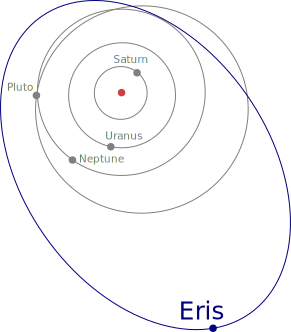
\includegraphics[width=0.5\textwidth]{img/eris-orbit}
  \caption{Orbit of the 136199 Eris dwarf planet}
  \label{fig:eris-orbit}
\end{figure}

Following this tradition, it seemed fitting to choose the name of the
dwarf planet Eris. Dwarf planets are neither planets not natural satellites,
but something in between. The name \Eris* beautifully encompasses the name of
the \gls{DWARF} debugging information format, and the fact that it is an
entity that is almost a moon


\tikzstyle{component} = [
  draw=black,
  thick,
  fill=green!10,
  rectangle,
  text centered,
  minimum height=2em,
  text width=6em,
  rounded corners,
  drop shadow,
]
\tikzstyle{uses} = [
  draw,
  very thick,
  >=triangle 45,
  ->,
  dashed,
]
\tikzstyle{contains} = [
  draw,
  thick,
  >=triangle 45,
  -*,
]

\begin{figure}
  \centering
  \begin{tikzpicture}[node distance=2cm]

    \node[component] (library) {Library};
    \node[component] (typecache) [above of=library]   {Type Cache};
    \node[component] (ctype)     [right=1cm of library]   {CType};
    \node[component] (function)  [right=1cm of ctype]     {Function};
    \node[component] (variable)  [right=1cm of function]  {Variable};
    \node[component] (typeinfo)  [above of=function]  {Type Information};
    \node[datain]    (dwarf)     [above=1cm of typecache]
                                  {DWARF debugging information};

    \node (luadata) [below right of=ctype] {Visible in Lua as userdata};
    \node (elf)     [above=0cm of dwarf]   {ELF shared object};

    \path[uses] (function) -- (typeinfo);
    \path[uses] (variable) -- (typeinfo);
    \path[uses] (ctype) -- (typeinfo);
    \path[uses] (typecache) -- (dwarf);
    \path[contains] (library) -- (typecache);
    \path[contains] (typecache) -- (typeinfo);

    \begin{pgfonlayer}{background}
      \node[datablob] (elfbox) [fit=(dwarf) (elf), drop shadow] {};
      \node[fill=yellow!20, rectangle, rounded corners] (wrappers)
      [fit=(library) (variable) (function) (luadata)] { };
    \end{pgfonlayer}
  \end{tikzpicture}
  \caption{Architecture of \Eris*.}
  \label{fig:eris-architecture}
\end{figure}
